%Baseado em
% https://www.overleaf.com/latex/templates/cse-3500-algorithms-and-complexity-homework-template/wrfwdhfzpnqc
\documentclass[12pt,letterpaper]{article}
\usepackage[top=2cm, bottom=4.5cm, left=2.5cm, right=2.5cm]{geometry}
\usepackage{amsmath,amsthm,amsfonts,amssymb,amscd}
\usepackage{enumerate}
\usepackage{fancyhdr}
\usepackage{mathrsfs}
\usepackage{xcolor} \usepackage{graphicx}
\usepackage{listings}
\usepackage{hyperref}
\usepackage{multicol}
\usepackage{xspace}
\usepackage{graphicx}

\usepackage[brazilian]{babel}

\hypersetup{%
  colorlinks=true,
  linkcolor=blue,
  linkbordercolor={0 0 1}
}

\setlength{\parindent}{0.0in}
\setlength{\parskip}{0.05in}

% Edit these as appropriate
\newcommand\course{ACH2016-102-2022}
\newcommand\prof{Valdinei Freire da Silva}
\newcommand\hwnumber{1}                   % <-- homework number
\newcommand\NUSP{11796083}                % <-- NUSP
\newcommand\sname{Henrique Tsuyoshi Yara}               % <-- Name

\newcommand\answer{\textbf{Resolução.}\xspace}

\pagestyle{fancyplain}
\headheight 35pt
\lhead{\sname \\ \NUSP}
\chead{\textbf{\Large Lista \hwnumber}}
\rhead{\course\, - \prof \\ \today}       % \today deixa o dia de hoje automaticamente
\lfoot{}
\cfoot{}
\rfoot{\center\small\thepage}
\headsep 1.5em

\graphicspath{ {./images} }

\begin{document}

% Use \section*{} em vez de \section{} para evitar que o Latex numere as
% seções. Isso evita que fique redundante "1 Exercício 1", por exemplo.
\section*{Exercício 1}

\[
    H \left( \mathcal{X} \right) = \sum_{i = 1}^{n} p(x_i) \log_2 \left( \frac{1}{p(x_i)} \right).
\]

%%%%%%%% ITEM 1.1 %%%%%%%%
\subsection*{1.a}

Represente os dados em um plano cartesiano com símbolos ou cores diferentes para cada categoria:

\answer \\

\begin{figure}[h]
	\center
	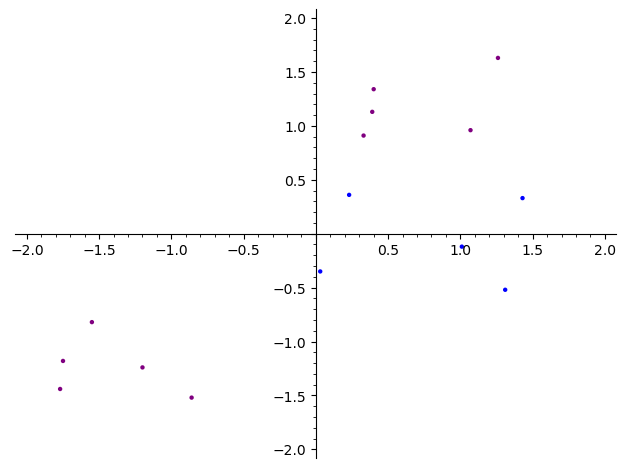
\includegraphics{ ex_1_1.png }
\end{figure}

%%%%%%%% FIM DO ITEM 1.1 %%%%%%%%

\subsection*{1.b}

Defina uma regra que classifique corretamente os exemplos da tabela.

\answer \\

Uma possível regra para classificar corretamente os exemplos da tabela seria:

\begin{equation}
	h(x_1, x_2) =
	\begin{pmatrix}
		\textrm{se} \quad x_1 > 0 \quad \textrm{e} \quad x_2 < 0.5 \quad \textrm{então} \quad 1 \\
		\textrm{se não} \quad 0 \\
	\end{pmatrix}
\end{equation}

\section*{Exercício 2}

\subsection*{2.a}

Calcule a entropia do conjunto de treinamento

\answer \\

A entropia do conjunto de treinamento pode ser calculado usando a fórmula:

\[
	H(V) = - (\frac{10}{15}\log_2\frac{10}{15} + \frac{5}{15}\log_2\frac{5}{15})
\]

Aplicando a fórmula:

$H(V) = - (\frac{10}{15}\log_2\frac{10}{15} + \frac{5}{15}\log_2\frac{5}{15})$

$H(V) = - (\frac{10}{15}-0.58496250072 + \frac{5}{15}-1.5849625007)$

$H(V) = - (\frac{2}{3}-0.58496250072 + \frac{1}{3}-1.5849625007)$

$H(V) = - (-0.389975 -0.528320833)$

$H(V) = - (-0.389975 -0.528320833)$

$H(V) = 0.918295833$

\subsection*{2.b - Errado}

Considere a pergunta $x_1 > 0$ e calcule a entropia média após obter a resposta a essa pergunta.

\answer \\

PS: Calculei quando $x_1 > 1$, corrigir depois

A entropia do conjunto de treinamento pode ser calculado usando a fórmula:

\[
	H(V) = - (\frac{2}{5}\log_2\frac{2}{5} + \frac{3}{5}\log_2\frac{3}{5})
\]

Aplicando a fórmula:

$H(V) = - (\frac{2}{5}\log_2\frac{2}{5} + \frac{3}{5}\log_2\frac{3}{5})$

$H(V) = - (\frac{2}{5}-1.3219280949 + \frac{3}{5}-0.73696559417)$

$H(V) = - (-0.528771237 -0.442179356)$

$H(V) = - (-0.528771237 -0.442179356)$

$H(V) = 0.970950593$

\subsection*{2.b}

Considere a pergunta $x_1 > 0$ e calcule a entropia média após obter a resposta a essa pergunta.

\answer \\

PS: Calculei quando $x_1 > 1$, corrigir depois

A entropia do conjunto de treinamento pode ser calculado usando a fórmula:

\[
	H(V) = - (\frac{5}{10}\log_2\frac{5}{10} + \frac{5}{10}\log_2\frac{5}{10})
\]

Aplicando a fórmula:

$H(V) = - (\frac{5}{10}\log_2\frac{5}{10} + \frac{5}{10}\log_2\frac{5}{10})$

$H(V) = - (\frac{2}{5}-1 + \frac{3}{5}-1)$

$H(V) = - (-\frac{2}{5} - \frac{3}{5})$

$H(V) = 1$

\subsection*{2.c}

Considere a pergunta $x_2 > 0$ e calcule a entropia média após obter a resposta a essa pergunta.

\answer \\

A entropia do conjunto de treinamento pode ser calculado usando a fórmula:

\[
	H(V) = - (\frac{5}{8}\log_2\frac{5}{8} + \frac{3}{8}\log_2\frac{3}{8})
\]

$H(V) = - (\frac{5}{8}\log_2\frac{5}{8} + \frac{3}{8}\log_2\frac{3}{8})$

$H(V) = - (\frac{5}{8}-0.67807190511 + \frac{3}{8}-1.4150374993)$

$H(V) = - (-0.42379494 -0.543890622)$

$H(V) = 0.967685562$

\subsection*{2.d}

Calcule os ganhos de informação obtidos para as duas respostas anteriores

\answer \\

Para calcular os ganhos de informação para as duas respostas anteriores, é possível usar a fórmula abaixo:

\[
	H(V) = - (\frac{5}{8}\log_2\frac{5}{8} + \frac{3}{8}\log_2\frac{3}{8})
\]



\subsection*{2.e}

Escolha a pergunta com maior ganho de informação para ser a raíz da árvore e complete a árvore para classificar corretamente todos os exemplos da tabela

\answer \\

\section*{Answers}

\begin{itemize}
	\item 2.a - $0,9183$
	\item 2.b - $0,667$
	\item 2.c - $0,9118$
	\item 2.d - $x_1 > 0 \rightarrow 0,2516$
	\item 2.d - $x_2 > 0 \rightarrow 0,0065$
	\item 3.c - $x_1 = 0,1076$
	\item 3.c - $x_2 = 0,6076$
	\item 4.e - $0,5027$
	\item 6.b - $\frac{10}{12}$
	\item 6.c - $\frac{7}{10}$
\end{itemize}

\end{document}
